\documentclass[]{article}
\usepackage{graphicx}
\usepackage[utf8]{inputenc}
\graphicspath{images/} 
\title{Chapter 10 - Question 8}
\author{Utkarsh Vardan}
\date{}
\begin{document}
\maketitle
Given buyers and sellers are as follows :\\
buyers : {a,b}\\
sellers:{x,y}\\\\
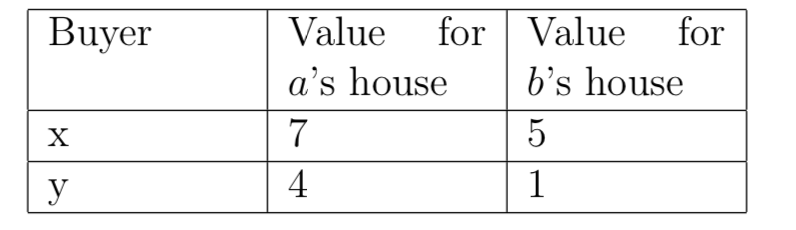
\includegraphics[scale=.5]{8q.png}\\
Let the initial price be 0 for each seller:\\\\\\\\\\
\textbf{Round1} 
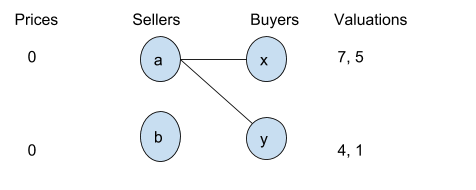
\includegraphics[scale=.5]{8r1.png}\\
Set of buyers X and Y are constricted to neighbour a,  This is not a perfect matching so seller a increases the price by 1 and the price of b remains 0.\\
The payoff for buyer x are as follows \\
a: (7-0)=7\\
b: (5-0)=5\\
The payoff of buyer y are as follows\\
a: (4-0)=4\\
b:(1-0)=1
\newpage
\textbf{Round2} \\
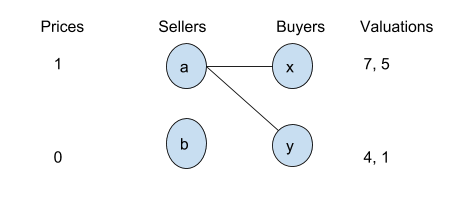
\includegraphics[scale=.5]{8r2.png}\\
Set of buyers X and Y are constricted to neighbour a,This is not perfect matching so seller a increases the price by 1 and the price of b remains 0.\\
The payoff for buyer x are as follows \\
a: (7-1)=6\\
b: (5-0)=5\\
The payoff of buyer y are as follows\\
a: (4-1)=3\\
b: (1-1)=0\\
\textbf{Round3} \\
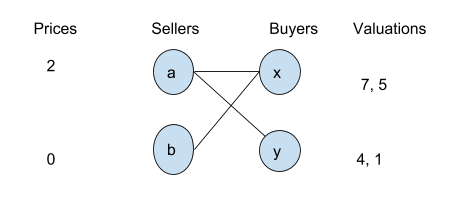
\includegraphics[scale=.5]{8r3.png}\\
We have perfect match now. Hence the current price 2 and 0 is the market clearing price.\\
The payoff for buyer x are as follows \\
a: (7-2)=5\\
b: (5-0)=5\\
The payoff of buyer y are as follows\\
a: (4-2)=2\\
b: (1-2)=-1\\
\\
\newpage
Chapter10 - Question 9
\newline
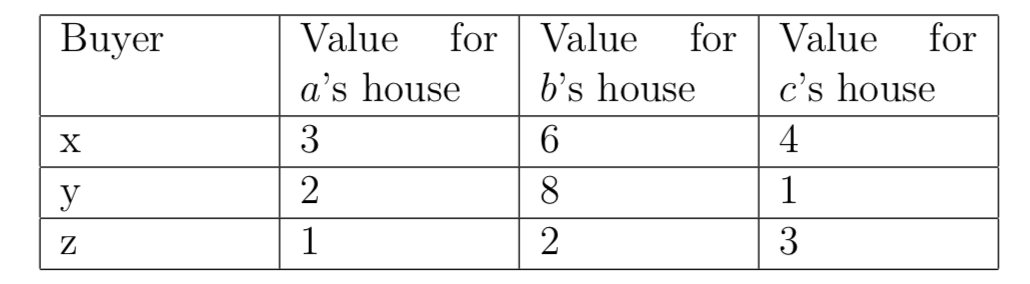
\includegraphics[scale=.5]{9q.png}\\\\
Given set of buyers and sellers are as follows:\\
Buyers {x, y, z}\\
Sellers {a,b,c}\\
Let the starting price for the sellers be 0.\\\\
\textbf{Round1}\\
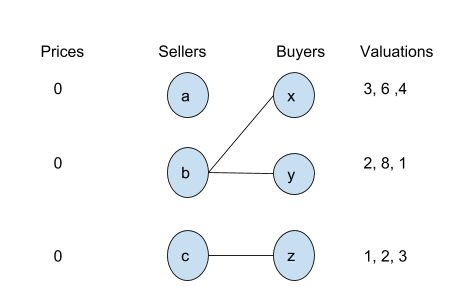
\includegraphics[scale=.5]{9r1.png}\\
Set of buyers consist of x and y forms a constricted set to the neighbour a. This is not a perfect matching. The price of b increases by 1 and the price of a and c remains 0.\\
The payoff for buyer x are as follows \\
a: (3-0)=3\\
b: (6-0)=6\\
c: (4-0)=4\\
The payoff of buyer y are as follows\\
a: (2-0)=2\\
b: (8-0)=8\\
c: (1-0)=1\\
The payoff of buyer z are as follows\\
a: (1-0)=1\
b: (2-0)=2\\
c: (3-0)=3\\
\newpage
\textbf{Round2}\\
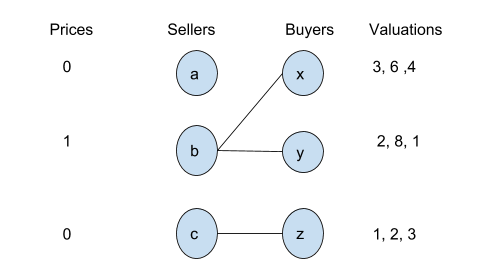
\includegraphics[scale=.5]{9r2.png}\\
Set of buyers consist of x and y forms a constricted set to the neighbour a. This is not a perfect matching. Only price of b increases by 1.\\\\
The payoff for buyer x are as follows \\
a: (3-0)=3\\
b: (6-1)=5\\
c: (4-0)=4\\
The payoff of buyer y are as \\
a: (2-0)=2\\
b: (8-1)=7\\
c: (1-0)=1\\
The payoff of buyer z are as follows\\
a: (1-0)=1\\
b: (2-1)=1\\
c: (3-0)=3\\
\textbf{Round3}\\
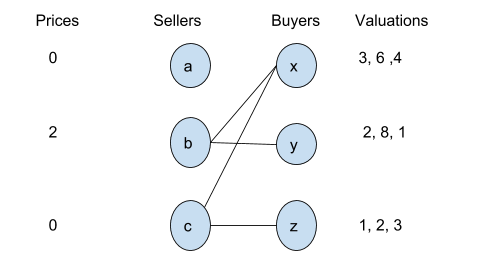
\includegraphics[scale=.5]{9r3.png}\\
Set of buyers consist of x, y and Z  forms a constricted set to the neighbour b and c. This is not a perfect matching. The price of b and c increases by 1 and the price of a and  remains 0.\\
The payoff for buyer x are as follows \\
a: (3-0)=3\\
b: (6-2)=4\\
c: (4-0)=4\\
The payoff of buyer y are as \\
a: (2-0)=2\\
b: (8-2)=6\\
c: (1-0)=1\\
The payoff of buyer z are as follows\\
a: (1-0)=1\\
b: (2-2)=0\\
c: (3-0)=3\\\\
\textbf{Round4}\\
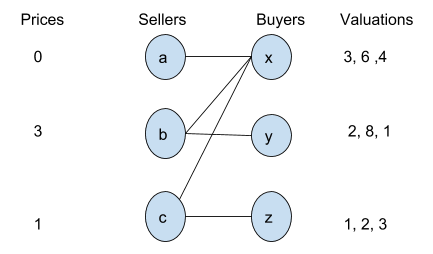
\includegraphics[scale=.5]{9r4.png}\\
We have a perfect match now. Hence the current price 0,3,1 are the marker clearing price\\
The payoff for buyer x are as follows \\
a: (3-0)=3\\
b: (6-3)=3\\
c: (4-1)=3\\
The payoff of buyer y are as \\
a: (2-0)=2\\
b: (8-3)=5\\
c: (1-1)=0\\
The payoff of buyer z are as follows\\
a: (1-0)=1\\
b: (2-3)=-1\\
c: (3-1)=2\\\\
\end{document}
